%!TEX TS-program = pdflatex
%!BIB program = biber
\documentclass[
wide,
% handout,
10pt,
xcolor={x11names,svgnames},
hyperref={pdfauthor={Jannes Bantje},colorlinks,urlcolor=maincolor,hidelinks=false,linkcolor=maincolor},
pantone312, 	% WWU-Design in hellblau
%pantone396, 	% WWU-Design in grellem hellgrün
%pantone315, 	% WWU-Design in dunkelblau
%pantone3282, 	% WWU-Design in "blau"
%pantone390, 	% WWU-Design in
%pantone369,	% WWU-Design in gras-grün
%pantoneblack7, % WWU-Design in dunklem gras-grün
%handout% aktivieren um \pause für Druck zu ignorieren (keine neue Seite für einen neuen Punkt)
euler-digits,
]{beamer}
\usepackage{etex}
% \usepackage{xxcolor}
% \definecolor{pantone312}{RGB}{0,157,209}
% \definecolor{maincolor}{named}{pantone312}
% \usepackage{newpxtext}
% \usepackage{palatino}
% \usepackage[bigdelims,varbb,varg]{newpxmath}

\usepackage{wwustyle2}
\usepackage{mathtools}
% \usepackage{newpxtext}
% \usepackage[bigdelims,varbb,varg]{newpxmath}
\usepackage{eulervm}
\usefonttheme{professionalfonts}

\usepackage[ngerman]{babel}
\usepackage{multirow}
\usepackage{booktabs}
\usepackage{xspace}

% -- Aufzählungen, Anführungszeichen etc.
% \usepackage[shortlabels,inline]{enumitem}
% % \setlist[itemize,1]{label=\faCaretRight}
% \setlist[enumerate]{font=\bfseries}
% \setlist{itemsep=0pt}
\usepackage[autostyle,german=quotes]{csquotes}

% \usepackage{array}

\AtBeginSection[]{
  \begin{frame}
  \vfill
  \centering
  \begin{beamercolorbox}[sep=8pt,center,shadow=true,rounded=true]{title}
    \usebeamerfont{title}\insertsectionhead\par%
  \end{beamercolorbox}
  \vfill
  \end{frame}
}

\newcommand{\aheader}[2]{\action<#1-|alert@#1>{#2}}
% first argument: slide number to appear from, second argument: content of header
\newcommand{\hiddencell}[2]{\action<#1->{#2}}
% first argument: slide number to appear from, second argument: content of cell

\DeclareRobustCommand{\GrpStruktur}{Gruppierungs-Struktur\xspace}

%-- um Inkompatibilitaeten von quotes und polyglossia bzw. babel zu vermeiden
\usepackage{tikz}
\usetikzlibrary{calc,fadings,decorations.pathreplacing,arrows.meta,arrows}

\tikzset{
  every picture/.append style={
    execute at begin picture={\shorthandoff{"}},
    execute at end picture={\shorthandon{"}}
  }
}
\usetikzlibrary{quotes}

\usepackage{eulervm}
\usepackage{mathtools} % beinhaltet amsmath
\usepackage{amssymb} % zusätzliche Symbole
% \usepackage{stmaryrd} % für Blitz
\usepackage{nicefrac} % schräge Brüche
\usepackage{faktor}
\newcommand{\Faktor}[1]{\faktor[\textstyle]{#1}}
\usepackage{xfrac}
\usepackage{cancel}
\usepackage{mathdots} % Verbesserung von Punkten wie zB \ldots
\usepackage[bb=px]{mathalfa}
\usepackage{centernot}


\usepackage{cleveref}

\newcommand{\Index}[1]{\bet{#1}}



\hypersetup{pdfstartview={Fit}}

\makeatletter
\renewcommand{\LaTeX}{L\kern -.22em{\sbox \z@ T\vbox to\ht \z@ {\hbox {\check@mathfonts \fontsize \sf@size \z@ \math@fontsfalse \selectfont A}\vss }}\kern -.10em\TeX}
\makeatother

\usepackage{multicol}


\newcommand{\bet}[1]{\textbf{\color{maincolor}#1}}
\newcommand{\keyword}[1]{{\color{pantone369}#1}}
\newcommand{\keyWWU}{\keyword{WWU Münster}\xspace}

%!TEX root = trajectory-grouping.tex

% -- Zum Finetuning von Befehlen
\makeatletter
\newcommand{\raisemath}[1]{\mathpalette{\raisem@th{#1}}}
\newcommand{\raisem@th}[3]{\raisebox{#1}{$#2#3$}}
\makeatother

% -- Box mit vorgegebener minimaler Länge
\DeclareRobustCommand{\minwidthbox}[2]{%
  \ifmmode
    \expandafter\mathmakebox
  \else
    \expandafter\makebox
  \fi
  [\ifdim#2<\width\width\else#2\fi]{#1}%
}

% -- farbiges Untersteichen im Mathe-Modus
\def\mathul#1#2{\color{#1}\underline{{\color{black}#2}}\color{black}} 


% -- besserer underbrace befehl
\newcommand{\Underbrace}[2]{{\underbrace{#1}_{#2}}}





%--Mengen
\newcommand\SetSymbol[1][]{\nonscript\:#1\vert\allowbreak\nonscript\:\mathopen{}}
\providecommand\given{} % to make it exist
\DeclarePairedDelimiterX\set[1]\{\}{\renewcommand\given{\SetSymbol[\delimsize]}#1}

% -- Betrag und Skalarprodukt
\DeclarePairedDelimiter{\abs}{\lvert}{\rvert}
\DeclarePairedDelimiterX\skal[2]{\langle}{\rangle}{#1\,,\,#2}

%--Umklammern
\DeclarePairedDelimiter\enbrace{(}{)}
\DeclarePairedDelimiter\benbrace{[}{]}
\DeclarePairedDelimiter\homo{\llbracket}{\rrbracket}
\newcommand{\ssbrace}[1]{{\scriptscriptstyle\enbrace{#1}}}

%--Norm
\DeclarePairedDelimiter\norm{\Vert}{\Vert}






% - verbessertes Integral
\newcommand{\Int}[1]{\int_{\mathrlap{#1}}\,\,}

% -- Alles spezielles aus der Differentialtopologie
\newcommand{\Tang}{\ensuremath{\mathrm{T}\mkern-0.85mu}}
\newcommand{\mathd}{\ensuremath{\mathrm{d}\mkern-0.7mu}}
\newcommand{\diff}[2]{\ensuremath{\frac{{\partial #1}}{{\partial #2}}}}
\newcommand{\diffs}[2]{\ensuremath{\partial #1/\partial #2}}
\newcommand{\diffd}[2]{\ensuremath{\frac{\mathd #1}{\mathd #2} }}
\DeclareMathOperator{\Lie}{L}
\DeclareMathOperator{\Ad}{Ad}  
\DeclareMathOperator{\ad}{ad}
\DeclareMathOperator{\Spin}{Spin}
% \DeclareMathOperator{\spin}{spin}
\newcommand{\spin}{\mathop{\mathfrak{spin}}}
\newcommand{\Ce}{\mathcal{C}}
\DeclareMathOperator{\vol}{vol}



%--Abbildungsdefinition
\newcommand{\mapdef}[5]{%
	\[
		\begin{array}{rcl}
			\textstyle #1 &\xrightarrow{\minwidthbox{#5}{2em}} & \textstyle #2 \\[0.5ex]
			\textstyle #3 &\xmapsto{\minwidthbox{\mbox{ }}{2em}} & \textstyle #4
		\end{array}
	\]
}

%--modifiziertes Stackrel
\newcommand{\StackText}[2]{\stackrel{\mbox{\scriptsize #1}}{#2}}
\newcommand{\StackTextClap}[2]{\stackrel{\mathclap{\mbox{\scriptsize #1}}}{#2}}





% -- theorem packages
\usepackage{amsthm}
% \theoremstyle{definition}
% \setbeamertemplate{theorems}[normal font]
\setbeamertemplate{theorems}[numbered]
\setbeamertemplate{definitions}[numbered]
% \renewtheorem{definition}{Definition}
\newtheorem{satz}{Satz}
\newtheorem{proposition}{Proposition}
\theoremstyle{definition}
\newtheorem{definitionP}{Definition \& Proposition}
% \theoremstyle{remark}
% \newtheorem{beweis}{Beweis}
\newenvironment{beweis}{\textsc{Beweis:}}{\qed}
\newenvironment{beweisX}{\textsc{Beweis:}}{}
\newenvironment{beweisCont}{\textsc{Beweis}(fortgesetzt):}{\qed}

% -- BibLaTeX
\usepackage[%
	backend=biber,
	sortlocale=auto,
	natbib,
	hyperref,
	backref,
	style=alphabetic,
	]%
{biblatex}
\renewcommand*{\mkbibnamefamily}[1]{%
  \ifmknamesc{\textsc{#1}}{#1}}

\renewcommand*{\mkbibnameprefix}[1]{%
  \ifboolexpr{ test {\ifmknamesc} and test {\ifuseprefix} }
    {\textsc{#1}}
    {#1}}

\def\ifmknamesc{%
  \ifboolexpr{ test {\ifcurrentname{labelname}}
               or test {\ifcurrentname{author}}
               or ( test {\ifnameundef{author}} and test {\ifcurrentname{editor}} ) }}
\addbibresource{quellen.bib}
\DefineBibliographyStrings{ngerman}{%
  andothers = {et\addabbrvspace al\adddot}
}
\setbeamertemplate{bibliography item}[text]


%-- Farben

\definecolor{blue3}{RGB}{27,53,62}
\definecolor{blue2}{RGB}{49,81,95}
\definecolor{blue1}{RGB}{84,113,121}
\definecolor{blueS}{RGB}{27,53,62}
\definecolor{teal3}{RGB}{34,107,96}
\definecolor{teal2}{RGB}{49,142,133}
\definecolor{teal1}{RGB}{77,165,154}
\definecolor{tealS}{RGB}{179,198,189}
\definecolor{red3}{RGB}{126,27,48}
\definecolor{red2}{RGB}{158,48,68}
\definecolor{red1}{RGB}{173,73,95}
\definecolor{redS}{RGB}{219,179,180}


\begin{document}
\makeatletter
\author{Jannes Bantje} \let\Author\@author
\title{Gruppierung von Trajektorien}
\subtitle{Seminar zur algorithmischen Geometrie}
\makeatother


\begin{frame}[plain]
  \maketitle
\end{frame}

\section{Einleitung}
\begin{frame}{Einleitung/Warum ist das interessant?}
    \begin{block}{Problemstellung}
        Gegeben eine Menge von $n$ Entitäten, die sich entlang gegebener Trajektorien bewegen, welche davon bewegen sich \enquote{zusammen}/in einer \enquote{Gruppe}?
    \end{block}\pause
    Zahlreiche mögliche Anwendungsgebiete:\pause
    \begin{itemize}[<+->]
        \item Bewegungen von Tieren in der Verhaltensbiologie (Herden und Rudel)
        \item Analyse von Verkehrsteilnehmern (z.B. zur Stau)
    \end{itemize}
    \onslide<5->{Bearbeitung der Problemstellung:}
    \begin{enumerate}
        \item<6-> Überführe menschliche Intuition einer kollektiven Bewegung in eine mathematische Definition
        \item<7-> Finde einen Weg, die so definierten \enquote{Gruppen} effektiv zu berechnen
    \end{enumerate}
\end{frame}

\begin{frame}{Ziel dieses Vortrags}
    \begin{center}
        \texttt{<Video hier>}
    \end{center}
\end{frame}

\begin{frame}{Tracectory Grouping Structure nach \textcite{buchin2015}}
    \begin{block}{Problemstellung}
        Gegeben eine Menge von $n$ Entitäten, die sich entlang gegebener Trajektorien bewegen, welche davon bewegen sich \enquote{zusammen}/in einer \enquote{Gruppe}?
    \end{block}
    Die \bet{Trajectory Grouping Structure} nach \textcite{buchin2015} zeichnet folgendes aus\pause
    \begin{itemize}[<+->]
        \item Intuitive Definition einer Gruppe von Trajektorien
        \item Neben der Identifikation von Gruppen wird auch das \enquote{Leben} von Gruppen betrachtet (Start, End, Merge und Split)
        \item Das Modell erfasst diese Änderungen der Gruppen zu kontinuierlichen Zeitpunkten
        \item Diese Struktur lässt sich effizient berechnen
        \item Gruppierung kann auf unterschiedlichen Maßstäben untersucht werden
        \item Das Modell kann robust gegenüber Störungen gemacht werden
    \end{itemize}
\end{frame}

\begin{frame}{Running Example: Skatenight in Münster}
    \begin{itemize}
        \item Der gesamte Zug (2500--3000 Personen) ist eine kollektive Bewegung
        \item Gruppierung lässt sich aber auch auf kleinerem Maßstab betrachten
    \end{itemize}
\end{frame}

\section{Definition einer Gruppe}

\begin{frame}{Was zeichnet eine kollektive Bewegung aus?}
    \begin{tabular}{rp{8cm}c}
        \hiddencell{2}{\bet{Räumliche Nähe} & Die einzelnen Entitäten dürfen nicht zu weit voneinander entfernt sein} & \hiddencell{5}{$\varepsilon \ge 0$}\\
        \hiddencell{3}{\bet{Mindestgröße} & In den meisten Anwendungsfällen sollten einzelne Entitäten keine Gruppe bilden} & \hiddencell{6}{$m \in \mathbb{N}$} \\
        \hiddencell{4}{\bet{Dauer} & eine kurze Begegnung von Entitäten sollte keine gemeinsame Bewegung sein} & \hiddencell{7}{$\delta \ge 0$} \\
    \end{tabular}
    \vspace{1em}

    \onslide<8->{Variation der Parameter ermöglicht:}
    \begin{itemize}
        \item<9-> Betonen bestimmter Aspekte (z.B. nur lange bestehende Gruppen durch großes $\delta$)
        \item<10-> Steuerung des Detailgrades, d.h. der Anzahl der Gruppen
    \end{itemize}
\end{frame}

\begin{frame}[t]{Räumliche Nähe}
    Sei $\mathcal{X}$ eine Menge von Entitäten, deren Ort innerhalb eines gewissen Zeitraums bekannt ist.\pause
    \begin{definition}<2->
        Zwei Entitäten $x$ und $y$ sind zum Zeitpunkt $t$ \bet{direkt zusammenhängend}, falls sich ihre $\varepsilon$-Bälle überlappen.
        
        $x$ und $y$ heißen \bet{$\varepsilon$-zusammenhängend} zum Zeitpunkt $t$, falls eine Folge von Entitäten $x=x_0, \ldots,x_k=y$ existiert, sodass $x_i$ und $x_{i+1}$ direkt zusammenhängend sind.
    \end{definition}
    \begin{columns}[c]
        \column{.65\textwidth}
        \begin{itemize}
            \item<3-> $\mathcal{S} \subseteq \mathcal{X}$ heißt \bet{Komponente} zum Zeitpunkt $t$, falls $S$ maximale $\varepsilon$-zusammenhängende Teilmenge ist.
            \item<4-> Mit $\mathcal{C}(t)$ bezeichnen wir die Menge der Komponenten zum Zeitpunkt $t$.
        \end{itemize}
        \column{.35\textwidth}
        \begin{tikzpicture}[scale=1.2]
			% \draw[help lines] (-1,-1) grid (2,2);
			\coordinate (1) at (0,-0.02);
			\coordinate (2) at (.05,.4);
			\coordinate (3) at (.5,.2);
			\coordinate (4) at (.85,-.08);
			\coordinate (5) at (1.45,-.04);
			\coordinate (6) at (-0.7,.3);
			\coordinate (7) at (2.1,.3);
			\coordinate (8) at (2.05,1);
			\coordinate (9) at (0.2,1.1);
			\coordinate (10) at (.9,-.65);
			\coordinate (11) at (2.2,.6);
			\coordinate (12) at (-.3,1);
			\coordinate (13) at (-.8,.9);
			\coordinate (14) at (-1.1,.5);
            \foreach \x in {1,2,...,14}{
				\draw[white,fill=white,fill opacity=.35,very thick] (\x) circle[radius=.4];
				% \draw[fill,very thick] (\x) circle[radius=.02];
			}
			\only<5>{\foreach \x in {1,2,...,14}{
				\draw[DodgerBlue3,fill=DodgerBlue3,fill opacity=.35,very thick] (\x) circle[radius=.4];
				\draw[fill,very thick] (\x) circle[radius=.02];
			}}
            \only<6>{
            \foreach \x in {1,2,...,5,10}{
				\draw[DodgerBlue3,fill=DodgerBlue3,fill opacity=.35,very thick] (\x) circle[radius=.3];
				\draw[fill,very thick] (\x) circle[radius=.02];
			}
			\foreach \x in {6,9,12,13,14}{
				\draw[Firebrick2,fill=Firebrick2,fill opacity=.35,very thick] (\x) circle[radius=.3];
				\draw[fill,very thick] (\x) circle[radius=.02];
			}
			\foreach \x in {7,8,11}{
				\draw[SeaGreen3,fill=SeaGreen3,fill opacity=.35,very thick] (\x) circle[radius=.3];
				\draw[fill,very thick] (\x) circle[radius=.02];
			}}
		\end{tikzpicture}
    \end{columns}
\end{frame}

\begin{frame}{Gruppen}
    \begin{definition}[Gruppe]
    	Eine Menge $G$ von $k$ Entitäten bildet eine \Index{Gruppe} im Zeitintervall $I$, falls gilt:
    	\begin{enumerate}[(i)]
    		\item $G$ enthält mindestens $m$ Entitäten, also $k \ge m$,
    		\item die Länge von $I$ ist mindestens $\delta$ und
    		\item zu jeder Zeit $t \in I$ existiert eine Komponente $C \in \mathcal{C}(t)$ mit $G \subseteq C$.
    	\end{enumerate}
    	Das Intervall $I=[t_s,t_e]$ der Gruppe $G$ bezeichnen wir auch mit $I_G$.
    	Eine Gruppe $H$ \bet{überlagert} $G$, falls $G \subseteq H$ und $I_G \subseteq I_H$ gilt.
    	Falls kein solches $H$ existiert, so heißt $G$ \bet{maximal}.
    \end{definition}\pause
    Es liegen folgende Monotonieeigenschaften vor:\pause
    \begin{itemize}[<+->]
        \item Verringern von $m$ und $\delta$: bestehende Gruppen bleiben erhalten und maximale Gruppen bleiben maximal.
        \item Vergrößern von $\varepsilon$:
        Gruppen bleiben erhalten, sind aber ggf. in größeren enthalten
        \item[$\Rightarrow$] detaillierte Sicht erhält maximale Gruppen, diese dehnen sich ggf. in Größe und Dauer aus
    \end{itemize}
\end{frame}

\begin{frame}{Beispiel maximaler Gruppen}
    \begin{center}
        \begin{tikzpicture}[scale=1.3]
    		% Zeitpunkte definieren
    		\coordinate (t_0) at (0,0);
    		\coordinate (t_1) at (2,0);
    		\coordinate (t_2) at (3.2,0);
    		\coordinate (t_3) at (4.5,0);
    		\coordinate (t_4) at (5.7,0);
    		\coordinate (t_5) at (6.2,0);
    		
    		\draw[gray,very thick] ($(t_0) - (.2,0)$) -- ($(t_5) + (.2,0)$);
    		\foreach \x in {t_0,t_1,t_2,t_3,t_4,t_5}{
    			\draw[gray, thick] ($(\x) + (0,.1)$) -- ($(\x)- (0,.1)$) node[below]{$\x$};
    		}
    		
    		% Trajektorien
    		\coordinate (0x_1) at ($(t_0) + (0,3)$);
    		\coordinate (1x_1) at ($(t_1) + (0,2.7)$);
    		\coordinate (2x_1) at ($(t_2) + (0,2.9)$);
    		\coordinate (3x_1) at ($(t_3) + (0,2.85)$);
    		\coordinate (4x_1) at ($(t_4) + (0,3.7)$);
    		\coordinate (5x_1) at ($(t_5) + (0,3.4)$);
    		               
    		\coordinate (0x_2) at ($(t_0) + (0,2.8)$);
    		\coordinate (1x_2) at ($(t_1) + (0,2.6)$);
    		\coordinate (2x_2) at ($(t_2) + (0,2.8)$);
    		\coordinate (3x_2) at ($(t_3) + (0,2.77)$);
    		\coordinate (4x_2) at ($(t_4) + (0,2.35)$);
    		\coordinate (5x_2) at ($(t_5) + (0,2.4)$);
    		               
    		\coordinate (0x_3) at ($(t_0) + (0,.8)$);
    		\coordinate (1x_3) at ($(t_1) + (0,1)$);
    		\coordinate (2x_3) at ($(t_2) + (0,2.7)$);
    		\coordinate (3x_3) at ($(t_3) + (0,2.68)$);
    		\coordinate (4x_3) at ($(t_4) + (0,2.2)$);
    		\coordinate (5x_3) at ($(t_5) + (0,2.35)$);
    		               
    		\coordinate (0x_4) at ($(t_0) + (0,.65)$);
    		\coordinate (1x_4) at ($(t_1) + (0,.9)$);
    		\coordinate (2x_4) at ($(t_2) + (0,1.3)$);
    		\coordinate (3x_4) at ($(t_3) + (0,.4)$);
    		\coordinate (4x_4) at ($(t_4) + (0,2.05)$);
    		\coordinate (5x_4) at ($(t_5) + (0,2.28)$);
    		
    		\foreach \x/\y in {x_1/DodgerBlue3,x_2/Firebrick2,x_3/SeaGreen3,x_4/Sienna2}{
    			\draw[very thick,\y] (0\x) node[left=1.4ex]{$\x$} -- (1\x) -- (2\x) -- (3\x) -- (4\x) -- (5\x);
    		}
    		
    		% epsilon-discs
    		\foreach \x in {x_1,x_2,x_3,x_4}{
    			\foreach \n in {0,1,...,5}{
    				\draw[darkgray,fill=gray,fill opacity=.2] (\n\x) circle[radius=.107];
    			}
    		}
    	\end{tikzpicture}
    \end{center}
    Maximalen Gruppen: \pause
    $\set*{x_1,x_2}$ während $[t_0,t_3]$, \pause
    $\set*{x_1,x_2,x_3}$ während $[t_2,t_3]$, \pause
    $\set*{x_2,x_3}$ während $[t_2,t_5]$, \pause
    $\set*{x_3,x_4}$ während $[t_0,t_1]$ \pause
    und $\set*{x_2,x_3,x_4}$ während $[t_4,t_5]$.
    % Hier wurde $m=2$ und $\delta < \abs*{t_5 - t_4}$ gewählt.
    % Wählt man stattdessen $\abs*{t_1-t_2}\ge \delta > \abs*{t_5 -t_4}$, so fällt die Gruppe $\set*{x_2,x_3,x_4}$ weg.
\end{frame}

\begin{frame}
    Weiterer Verlauf:
    \begin{itemize}[<+->]
        \item Definition des sog. \bet{Reeb-Graphen}
        \item Definition der sog. \bet{\GrpStruktur} bestehend aus der Menge der maximalen Gruppen und dem \bet{Reeb-Graphen}
        \item Komplexität der \GrpStruktur
        \item Berechnung der \GrpStruktur
    \end{itemize}
\end{frame}

\section{Der Reeb-Graph}

\begin{frame}{Reeb-Graph}
    Sei $X$ ein topologischer Raum und $f \colon X \to \mathbb{R}$ stetig, wobei wir uns $f$ als Höhenfunktion vorstellen.
    \begin{definition}<2->[Reeb-Graph]
    	Der \bet{Reeb-Graph} zu $f \colon X \to \mathbb{R}$ ist der Quotientenraum $\mathcal{R}(f) \coloneqq X/{\sim}$ bezüglich der folgenden Äquivalenzrelation
    	\[
    		x \sim y \,:\mkern-3mu\iff \exists a \in \mathbb{R} : x,y \text{ liegen in der gleichen Zsmh.-Komponente von } f^{-1}(\set{a})
    	\]
    	Die Elemente von $\mathcal{R}(f)$ bezeichnen wir als \Index{Konturen} von $f$.
    \end{definition}
    \begin{itemize}
        \item<3-> Auf jeder Höhe werden also die Zusammenhangskomponenten zu einem Punkt kollabiert
        \item<4-> Es ist \emph{a priori} überhaupt nicht klar, dass $\mathcal{R}(f)$ ein Graph ist!
        \item<5-> Insbesondere ist nicht klar, welche Punkte aus $x$ auf Knoten in $\mathcal{R}(f)$ abgebildet werden.
        \item<6-> $\mathcal{R}(f)$ ist gerichtet (induziert durch die positive Richtung in $\mathbb{R}$)
    \end{itemize}
\end{frame}

\begin{frame}{Beispiel: Reeb-Graph des aufrechten Torus}
    \centering
    \begin{tikzpicture}[rotate=90, xscale=1, yscale=1, scale=0.7]
		% \draw[help lines] (-4,-10) grid (4,4);
		% reelle Gerade
		\draw[->,thick] (-4,-6) -- ++ (8,0) node[left=3pt]{$\mathbb{R}$};
		
        \only<3->{
		\draw[DodgerBlue3, thick] (-2.5,1.89) .. controls +(240:0.8) and +(120:0.8) .. (-2.5,-1.89);
		\draw[DodgerBlue3, thick, dashed] (-2.5,1.89) .. controls +(300:0.8) and +(60:0.8) .. (-2.5,-1.89);
		\draw[fill=DodgerBlue3] (-2.5,-6) circle[radius=0.09];
		}
        
        \only<5->{
		\draw[Firebrick2, thick] (0,2.5) .. controls +(250:0.6) and +(110:0.6) .. (0,0.5);
		\draw[Firebrick2, thick, dashed] (0,2.5) .. controls +(290:0.6) and +(70:0.6) .. (0,0.5);
		
		\draw[Firebrick2, thick] (0,-0.5) .. controls +(250:0.6) and +(110:0.6) .. (0,-2.5);
		\draw[Firebrick2, thick, dashed] (0,-0.5) .. controls +(290:0.6) and +(70:0.6) .. (0,-2.5);
		\draw[fill=Firebrick2] (0,-6) circle[radius=0.09];
        }
		
        \only<6->{
		\draw[SeaGreen3, thick] (1.75,2.25) .. controls +(250:0.6) and +(110:0.6) .. (1.75,0) .. controls +(250:0.6) and +(110:0.6) .. (1.75,-2.25);
		\draw[SeaGreen3, thick, dashed] (1.75,2.25) .. controls +(290:0.6) and +(70:0.6) .. (1.75,0) .. controls +(290:0.6) and +(70:0.6) .. (1.75,-2.25);
		\draw[fill=SeaGreen3] (1.75,-6) circle[radius=0.09];
        }
		
        \only<4->{
		\draw[SeaGreen3, thick] (-1.75,2.25) .. controls +(250:0.6) and +(110:0.6) .. (-1.75,0) .. controls +(250:0.6) and +(110:0.6) .. (-1.75,-2.25);
		\draw[SeaGreen3, thick, dashed] (-1.75,2.25) .. controls +(290:0.6) and +(70:0.6) .. (-1.75,0) .. controls +(290:0.6) and +(70:0.6) .. (-1.75,-2.25);
		\draw[fill=SeaGreen3] (-1.75,-6) circle[radius=0.09];
		}
		% kritische Werte and Start und Ende
		\begin{scope}
			\clip (-3.5,-1) rectangle (3.5,1);
			\only<7->{\draw[Sienna2,fill=Sienna2] (3.5,0) circle[radius=.08];}
			\only<2->{\draw[Sienna2,fill=Sienna2] (-3.5,0) circle[radius=.08];}
		\end{scope}
		\only<7->{\draw[fill=Sienna2] (3.5,-6) circle[radius=.09];}
		\only<2->{\draw[fill=Sienna2] (-3.5,-6) circle[radius=.09];}
		
		% draw reeb graph
        \begin{scope}[every node/.style={shape=circle,inner sep=1.7pt,fill=white}]
			\draw[thick,white] (-3.5,-12) node{} -- ++(1.75,0) .. controls +(80:1.5) and +(100:1.5) .. ++(3.5,0) node{};
			\draw[thick,white] (3.5,-12) node{}-- ++(-1.75,0) .. controls +(-100:1.5) and +(-80:1.5) .. ++(-3.5,0) node{};
		\end{scope}
        
		\begin{scope}[every node/.style={shape=circle,inner sep=1.7pt,fill}]
            \only<1>{\clip (-3.7,-10) rectangle (-3.7,-14); }
            \only<2>{\clip (-3.7,-10) rectangle (-3.3,-14); }
            \only<3>{\clip (-3.7,-10) rectangle (-2.5,-14); }
            \only<4>{\clip (-3.7,-10) rectangle (-1.6,-14); }
            \only<5>{\clip (-3.7,-10) rectangle (0,-14); }
            \only<6>{\clip (-3.7,-10) rectangle (1.9,-14); }
            \only<7>{\clip (-3.7,-10) rectangle (3.5,-14); }
            \only<8>{\clip (-3.7,-10) rectangle (3.7,-14); }
			\draw[thick] (-3.5,-12) coordinate (a1) -- ++(1.75,0) coordinate (a2) .. controls +(80:1.5) and +(100:1.5) .. ++(3.5,0) coordinate (a3);
			\draw[thick] (3.5,-12) coordinate (a4) -- ++(-1.75,0) .. controls +(-100:1.5) and +(-80:1.5) .. ++(-3.5,0);
            \only<8->{\foreach \x in {1,2,3,4}{
                \draw (a\x) node{};
            }}
		\end{scope}
        
		\node at (4,-11) {$\mathcal{R}(f)$};
		
		\draw[thick] (-3.5,0) .. controls (-3.5,2) and (-1.5,2.5) .. (0,2.5);
		\draw[thick,xscale=-1] (-3.5,0) .. controls (-3.5,2) and (-1.5,2.5) .. (0,2.5);
		\draw[thick,rotate=180] (-3.5,0) .. controls (-3.5,2) and (-1.5,2.5) .. (0,2.5);
		\draw[thick,yscale=-1] (-3.5,0) .. controls (-3.5,2) and (-1.5,2.5) .. (0,2.5);
		\draw[thick] (-2,.2) .. controls (-1.5,-0.3) and (-1,-0.5) .. (0,-.5) .. controls (1,-0.5) and (1.5,-0.3) .. (2,0.2);
		\draw[thick] (-1.75,0) .. controls (-1.5,0.3) and (-1,0.5) .. (0,.5) .. controls (1,0.5) and (1.5,0.3) .. (1.75,0);
		
		\draw[-to] (0,-3.5) -- (0,-5) node[above, midway]{$f$};
	\end{tikzpicture}
    % \uncover<9->{Die grünen und orangenen Punkte sind die kritischen Werte von $f$.}
\end{frame}

\begin{frame}{Identifikation der Knoten im Reeb-Graph}
    Wo kommen die Knoten im Reeb-Graph $\mathcal{R}(f)$ her? \pause
    % Unter folgenden Zusatzannahmen können die Knoten in $\mathcal{R}(f)$ leicht charakterisiert werden
    \begin{itemize}[<+->]
        \item Unter Zusatzannahmen ist eine mathematisch zufriendenstellende Antwort möglich
        \item Dafür muss $X$ eine Mannigfaltigkeit und $f \colon X \to \mathbb{R}$ eine sog. Morse-Funktion sein
        \item Zentrale Erkenntnis der Morse-Theorie: Die Topologie von $X$ ändert sich nur an den \bet{kritischen Werten} von $f$!
        \item Folglich können sich die Zusammenhangskomponenten der Niveaumengen auch nur an kritischen Werten ändern
        \item[$\Rightarrow$] Bijektion zwischen Knoten in $\mathcal{R}(f)$ und kritischen Punkten von $f$
    \end{itemize}\pause
    Weitere Details: Siehe Ausarbeitung, \textcite{compTopo}, \textcite{MilnorMorse} \pause\vspace{1em}
    \begin{center}
        \large Und nun zurück zu unseren Trajektorien \ldots
    \end{center}
\end{frame}

\begin{frame}{Reeb-Graph zu einer Menge von Trajektorien}
    Sei $\mathcal{X}$ wieder die Menge der Entitäten, von denen sich jede entlang einer Trajektorie aus $\tau$ Kanten bewegt.
    \begin{itemize}
        \item Extrusion der $\varepsilon$-Scheibe um $x$ über die Zeit liefert eine Teilmenge $\mathcal{M}_x \subseteq \mathbb{R}^3$ zusammengesetzt aus schiefen Zylindern
        \item Vereinigen liefert Raum $\mathcal{M} \coloneqq \bigcup_{x \in \mathcal{X}} \mathcal{M}_x  \subseteq \mathbb{R}^3$, dessen Reeb-Graph wir betrachten wollen
        \item Sei $H_t$ horizontale Ebene zum Zeitpunkt $t$, dann ist $\mathcal{M} \cap H_t$ Niveaumenge und Zusammenhangskomponenten von $\mathcal{M} \cap H_t$ entsprechen Komponenten im Sinne von Definition 1.
    \end{itemize}
    \begin{definition}
        Wir bezeichnen mit $\mathcal{R}$ den Reeb-Graph zu $\mathcal{M}$ bezüglich der $z$-Höhenfunktion.
    \end{definition}
\end{frame}

\begin{frame}[t]{Beispiel: Reeb-Graph von $\mathcal{M}$}
    \begin{center}
        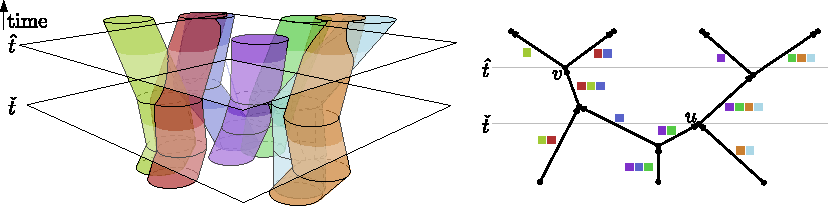
\includegraphics[width=1.05\textwidth]{Bilder/manifold.pdf}
        \mbox{ }\hfill {\small Quelle: \cite[Fig.~2]{buchin2015}}\pause
        \begin{itemize}[<+->]
            \item $\mathcal{M}$ ist eine 3-dimensionale Mannigfaltigkeit mit Rand \textcolor{gray}{in den meisten Fällen}
            \item Der Reeb-Graph beschreibt, wie sich die Komponenten mit der Zeit verändern
        \end{itemize}
    \end{center}
\end{frame}

\begin{frame}{Knoten des Reeb-Graphen}
    \begin{columns}
        \column{.6\textwidth}
        \begin{itemize}[<+->]
            \item Annahmen im weiteren Verlauf:
            \begin{itemize}
                \item Die bekannten Positionen der Trajektorien sind alle an gleichen Zeitpunkten $t_0, \ldots ,t_\tau$.
            	\item Keine drei Entitäten werden zur gleichen Zeit $\varepsilon$-(un)zusammenhängend.
            \end{itemize}
            \item Damit können wir die Knoten des Reeb-Graphen in vier Typen unterteilen.
            \item Jeder Kante lassen sich die zugehörigen Entitäten und Gruppen zuordnen.
            \item Wenn $\delta>0$ oder $m>1$, so \enquote{reduziere} $\mathcal{R}$.
        \end{itemize}
        \begin{definition}<7->
            Die \bet{Trajectory Grouping Structure} zu $\mathcal{X}$ ist $\mathcal{R}$ zusammen mit einer Abbildung, die jeder Kante die zugehörige Menge maximaler Gruppen zuordnet.
        \end{definition}
        \column{.36\textwidth}
        % \centering
        \uncover<4->{\begin{tabular}{lcc}
            \toprule
            Typ & In-Degree & Out-Degree \\
            \midrule
            Start & 0 & 1\\
            End & 1 & 0\\
            Merge & 2 & 1\\
            Split & 1 & 2\\
            \bottomrule
        \end{tabular}}\\[4em]
        \uncover<4->{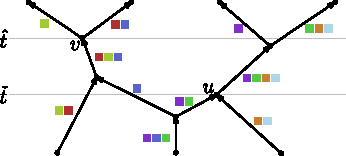
\includegraphics[width=1.1\textwidth]{Bilder/manifold_right.pdf}}
    \end{columns}
\end{frame}

\section{Komplexität der Gruppierungsstruktur}
\label{sec:Komplexität der Gruppierungsstruktur}

\begin{frame}{Komplexität des Reeb-Graphen}
    \begin{lemma}[{\cite[Lem.~1]{buchin2015}}]
    	Der Reeb-Graph $\mathcal{R}$ einer Menge $\mathcal{X}$ von $n$ Entitäten, von denen sich jede auf einer Trajektorie mit $\tau$ Kanten bewegt, kann $\Omega(\tau n^2)$ Vertices und $\Omega(\tau n^2)$ Kanten haben.
    \end{lemma}
    \begin{columns}
        \column[T]{.45\textwidth}
        \centering
        \begin{tikzpicture}[scale=.25,>=Latex,font=\small]
            \only<3->{
			\draw[dashed] (-7,-7) node[left]{$t_i$} -- (7,7);
			\draw[dashed] (0,-12) node[left]{$t_{i+1}$} -- ++ (14,14);
            }
			\foreach \x in {1,2,3,4,5}{
                \only<3>{
                \path (-\x,-\x) node[left]{$r_{\x}$} ;
                \path (\x,\x) node[above,xshift=-1pt]{$d_{\x}$} ;
                }
                \only<4->{
				\draw[->,thick] (-\x,-\x) node[left]{$r_{\x}$} -- ++ (12,0);
				\draw[->,thick] (\x,\x) node[above,xshift=-1pt]{$d_{\x}$} -- ++ (0,-12);
                }
                \only<3>{
				\filldraw[fill=DodgerBlue3] (-\x,-\x) circle[radius=.15];
				\filldraw[fill=Firebrick2] (\x,\x) circle[radius=.15];
                }
                \only<4->{
				\filldraw[fill=DodgerBlue3] (-\x,-\x) circle[radius=.15] ++ (12,0)circle[radius=.15];
				\filldraw[fill=Firebrick2] (\x,\x) circle[radius=.15] ++ (0,-12) circle[radius=.15];
                }
			}
		\end{tikzpicture}
        \column[T]{.55\textwidth}
        \begin{beweis}
            \onslide<2->{O.B.d.A. sei $n$ gerade, wähle $\varepsilon=0$.}
            \begin{itemize}
                \item<3-> Teile auf: $\mathcal{X}= R \cup D$.
                \item<4-> In jedem Intervall $[t_i,t_{i+1}]$ bewegen sich die Entitäten, wie in nebenstehender Skizze in konstanter Geschwindigkeit.
                \item<5-> Während $[t_i,t_{i+1}]$ erzeugt jede Entität $d_j$ mit jeder Entität $r_\ell$ einen Knoten in $\mathcal{R}$
                \item<6-> Pro Zeitabschnitt also $\mathcal{O}(n^2)$ viele Knoten.
            \end{itemize}
            \onslide<7->{Es folgt die Behauptung, da der Knotengrad höchstens 3 ist.}
        \end{beweis}
    \end{columns}
\end{frame}

\begin{frame}{Komplexität des Reeb-Graphen II.}
    \begin{satz}[{\cite[Thm.~2]{buchin2015}}]
    	Der Reeb-Graph $\mathcal{R}=(V,E)$ aus dem vorigen Lemma hat $\mathcal{O}(\tau n^2)$ Vertices und Kanten.
    	Diese Schranke ist scharf im Worst-Case.
    \end{satz}
    \begin{beweis} \pause
        Mit dem vorigen Lemma muss nur gezeigt werden, dass der Reeb-Graph $\mathcal{O}(\tau n^2)$ Vertices und Kanten hat.\pause
        \begin{itemize}[<+->]
            \item Während eines Zeitabschnitts $[t_i,t_{i+1}]$ bewegen sich zwei Entitäten $x,y$ auf Geraden.
            \item Eine einfache Rechnung zeigt: Ihr Abstand wird währendessen durch eine konvexe Funktion beschrieben.
            \item Also sind $x$ und $y$ nur innerhalb höchstens eines Intervalls $I \subseteq [t_i,t_{i+1}]$ direkt zusammenhängend.
            \item Dies induziert höchstens zwei Knoten in $\mathcal{R}$ $\implies$ Für jedes Paar $x,y$ existieren $\mathcal{O}(\tau)$ Knoten in $\mathcal{R}$.
        \end{itemize}
        \onslide<7->{Damit folgt die Behauptung (wieder hat jeder Knoten konstanten Grad).}
    \end{beweis}
\end{frame}

\begin{frame}{Schranke für die Anzahl maximaler Gruppen}
    \pause
    \begin{itemize}[<+->]
        \item Erste Idee: Jeder Knoten in $\mathcal{R}$ erzeugt höchstens so viele maximale Gruppen, wie er ausgehende Kanten hat.
        \item Problem: Dass eine Gruppe maximal ist, kann man oft erst feststellen, wenn eine überlagernde maximale Gruppe endet
        \item Man kann Beispiele konstruieren, bei denen an einem Split-Knoten sehr viele maximale Gruppen entdeckt werden, siehe \cite[S.~81, Fig.~4]{buchin2015}.
        \item Mit etwas Aufwand lässt sich trotzdem folgendes beweisen:
    \end{itemize}
    \begin{satz}<6->[{\cite[Thm.~5]{buchin2015}}]
    	Für eine Menge $\mathcal{X}$ von $n$ Entitäten, von denen sich jede enthalt einer Trajektorie von $\tau$ Kanten bewegt, gibt es $\mathcal{O}(\tau n^3)$ maximale Gruppen.
    	Diese Schranke ist scharf im Worst-Case.
    \end{satz}
\end{frame}

\section{Berechung der Gruppierungsstruktur}
\label{sec:Berechung der Gruppierungsstruktur}

\begin{frame}{Berechung der Gruppierungsstruktur}
    \begin{itemize}
        \item Grundsätzliches Vorgehen:
        \begin{enumerate}
            \item Berechne den Reeb-Graphen $\mathcal{R}$
            \item Beschrifte die Kanten mit den maximalen Gruppen.
        \end{enumerate}
        \item Wie berechnet man den Reeb-Graphen?
        \item Eine Repräsentation von $\mathcal{M}$ will man auf keinen Fall generieren!
        \item Betrachte dazu noch einmal das Beispiel von vorhin \ldots
    \end{itemize}
\end{frame}

\begin{frame}{Erinnerung: Konstruktion des Reeb-Graphen zum Torus}
    \centering
    \begin{tikzpicture}[rotate=90, xscale=1, yscale=1, scale=0.7]
		% \draw[help lines] (-4,-10) grid (4,4);
		% reelle Gerade
		\draw[->,thick] (-4,-6) -- ++ (8,0) node[left=3pt]{$\mathbb{R}$};
		
        \only<3->{
		\draw[DodgerBlue3, thick] (-2.5,1.89) .. controls +(240:0.8) and +(120:0.8) .. (-2.5,-1.89);
		\draw[DodgerBlue3, thick, dashed] (-2.5,1.89) .. controls +(300:0.8) and +(60:0.8) .. (-2.5,-1.89);
		\draw[fill=DodgerBlue3] (-2.5,-6) circle[radius=0.09];
		}
        
        \only<5->{
		\draw[Firebrick2, thick] (0,2.5) .. controls +(250:0.6) and +(110:0.6) .. (0,0.5);
		\draw[Firebrick2, thick, dashed] (0,2.5) .. controls +(290:0.6) and +(70:0.6) .. (0,0.5);
		
		\draw[Firebrick2, thick] (0,-0.5) .. controls +(250:0.6) and +(110:0.6) .. (0,-2.5);
		\draw[Firebrick2, thick, dashed] (0,-0.5) .. controls +(290:0.6) and +(70:0.6) .. (0,-2.5);
		\draw[fill=Firebrick2] (0,-6) circle[radius=0.09];
        }
		
        \only<6->{
		\draw[SeaGreen3, thick] (1.75,2.25) .. controls +(250:0.6) and +(110:0.6) .. (1.75,0) .. controls +(250:0.6) and +(110:0.6) .. (1.75,-2.25);
		\draw[SeaGreen3, thick, dashed] (1.75,2.25) .. controls +(290:0.6) and +(70:0.6) .. (1.75,0) .. controls +(290:0.6) and +(70:0.6) .. (1.75,-2.25);
		\draw[fill=SeaGreen3] (1.75,-6) circle[radius=0.09];
        }
		
        \only<4->{
		\draw[SeaGreen3, thick] (-1.75,2.25) .. controls +(250:0.6) and +(110:0.6) .. (-1.75,0) .. controls +(250:0.6) and +(110:0.6) .. (-1.75,-2.25);
		\draw[SeaGreen3, thick, dashed] (-1.75,2.25) .. controls +(290:0.6) and +(70:0.6) .. (-1.75,0) .. controls +(290:0.6) and +(70:0.6) .. (-1.75,-2.25);
		\draw[fill=SeaGreen3] (-1.75,-6) circle[radius=0.09];
		}
		% kritische Werte and Start und Ende
		\begin{scope}
			\clip (-3.5,-1) rectangle (3.5,1);
			\only<7->{\draw[Sienna2,fill=Sienna2] (3.5,0) circle[radius=.08];}
			\only<2->{\draw[Sienna2,fill=Sienna2] (-3.5,0) circle[radius=.08];}
		\end{scope}
		\only<7->{\draw[fill=Sienna2] (3.5,-6) circle[radius=.09];}
		\only<2->{\draw[fill=Sienna2] (-3.5,-6) circle[radius=.09];}
		
		% draw reeb graph
        \begin{scope}[every node/.style={shape=circle,inner sep=1.7pt,fill=white}]
			\draw[thick,white] (-3.5,-12) node{} -- ++(1.75,0) .. controls +(80:1.5) and +(100:1.5) .. ++(3.5,0) node{};
			\draw[thick,white] (3.5,-12) node{}-- ++(-1.75,0) .. controls +(-100:1.5) and +(-80:1.5) .. ++(-3.5,0) node{};
		\end{scope}
        
		\begin{scope}[every node/.style={shape=circle,inner sep=1.7pt,fill}]
            \only<1>{\clip (-3.7,-10) rectangle (-3.7,-14); }
            \only<2>{\clip (-3.7,-10) rectangle (-3.3,-14); }
            \only<3>{\clip (-3.7,-10) rectangle (-2.5,-14); }
            \only<4>{\clip (-3.7,-10) rectangle (-1.6,-14); }
            \only<5>{\clip (-3.7,-10) rectangle (0,-14); }
            \only<6>{\clip (-3.7,-10) rectangle (1.9,-14); }
            \only<7>{\clip (-3.7,-10) rectangle (3.7,-14); }
            % \only<8>{\clip (-3.7,-10) rectangle (3.7,-14); }
			\draw[thick] (-3.5,-12) coordinate (a1) -- ++(1.75,0) coordinate (a2) .. controls +(80:1.5) and +(100:1.5) .. ++(3.5,0) coordinate (a3);
			\draw[thick] (3.5,-12) coordinate (a4) -- ++(-1.75,0) .. controls +(-100:1.5) and +(-80:1.5) .. ++(-3.5,0);
            \foreach \x in {1,2,3,4}{
                \draw (a\x) node{};
            }
		\end{scope}
        
		\node at (4,-11) {$\mathcal{R}(f)$};
		
		\draw[thick] (-3.5,0) .. controls (-3.5,2) and (-1.5,2.5) .. (0,2.5);
		\draw[thick,xscale=-1] (-3.5,0) .. controls (-3.5,2) and (-1.5,2.5) .. (0,2.5);
		\draw[thick,rotate=180] (-3.5,0) .. controls (-3.5,2) and (-1.5,2.5) .. (0,2.5);
		\draw[thick,yscale=-1] (-3.5,0) .. controls (-3.5,2) and (-1.5,2.5) .. (0,2.5);
		\draw[thick] (-2,.2) .. controls (-1.5,-0.3) and (-1,-0.5) .. (0,-.5) .. controls (1,-0.5) and (1.5,-0.3) .. (2,0.2);
		\draw[thick] (-1.75,0) .. controls (-1.5,0.3) and (-1,0.5) .. (0,.5) .. controls (1,0.5) and (1.5,0.3) .. (1.75,0);
		
		\draw[-to] (0,-3.5) -- (0,-5) node[above, midway]{$f$};
	\end{tikzpicture}
\end{frame}

\begin{frame}{Sweep zur Berechnung von $\mathcal{R}$}
    \begin{itemize}
        \item Frage: Wie diskretisiert man den Sweep?
        \item Anders formuliert: Wie sieht die Queue aus?
        \item Problem: Im Allgemeinen ändern sich die Komponenten nicht zu den Zeitpunkten $t_0, \ldots, t_\tau$, sondern dazwischen.
        \item Knoten im Reeb-Graph entsprechen kritischen Werten, also brauchen wir eigentlich nur ein Liste ebendieser
        \item Da sich diese nicht so einfach berechen lassen, nehmen wir folgende Obermenge:
    \end{itemize}
    \begin{block}{Queue}
        Liste aller \emph{Connect}- und \emph{Disconnect}-Ereignisse, d.h. sortierte Liste von Zeitpunkten an denen zwei Entitäten direkt (un)zusammenhängend werden.
    \end{block}
    \begin{itemize}
        \item Diese Liste mit $\mathcal{O}(\tau n^2)$ Ereignisse lässt sich in $\mathcal{O}(\tau n^2 \log n)$ Zeit berechnen.
    \end{itemize}
\end{frame}

\begin{frame}%{Die $xy$-Struktur}
    \begin{block}{$xy$-Struktur}
        \begin{itemize}
            \item Gewichteter Graph $G=(\mathcal{X},Z)$, der die \enquote{direkt zusammenhängend}-Relation repräsentiert
            \item Die Gewichte sind die Zeitpunkte, wann die Kante wieder entfernt wird.
            \item Maximaler Spannbaum $F$ zur Verwaltung der Zusammenhangskomponenten von $G$.
        \end{itemize}
    \end{block}
    \begin{itemize}
        \item Geschicktes Ausnutzen der Gewichte und geeignete Datenstruktur für $F$ ermöglicht Updates von $G$ und $F$ in $\mathcal{O}(\log n)$ Zeit, siehe Ausarbeitung bzw. \cites{buchin2015}{parsaReeb}.
        \item Bei der Behandlung der Ereignisse muss überprüft werden, ob die Änderung des direkten Zusammenhangs zweier Entitäten auch die Komponenten ändern.
    \end{itemize}
    \begin{satz}[{\cite[Thm.~7]{buchin2015}}]
    	Für eine Menge $\mathcal{X}$ von $n$ Entitäten, von denen sich jede entlang einer Trajektorie von $\tau$ Kanten bewegt, besteht der Reeb-Graph $\mathcal{R}$ aus $\mathcal{O}(\tau n^2)$ Knoten und Kanten und kann in $\mathcal{O}(\tau n^2 \log n)$ Zeit berechnet werden.
    \end{satz}
\end{frame}

\begin{frame}{Berechnung der maximalen Gruppen}
    \begin{itemize}
        \item Idee: Betrachte $\mathcal{R}$, berechne aus den bereits beschrifteten eingehenden Kanten Beschriftungen mit maximalen Gruppen für die ausgehenden Kanten.
        \item Traversiere $\mathcal{R}$ dazu in \bet{topologischer Reihenfolge}.
        \item Problematisch ist dabei die effiziente Behandlung von Split-Knoten.
        \item Lösung: Assoziiere zur jeder Kante in $\mathcal{R}$ einen Baum, um $\mathcal{R}$ nicht zusätzlich \enquote{rückwärts} traversieren zu müssen.
        \item Details: Ausarbeitung und \textcite{buchin2015}
    \end{itemize}
    \begin{satz}[{\cite[Thm.~9]{buchin2015}}]
        Alle maximalen Gruppen lassen sich in $\mathcal{O}(\tau n^3 + N)$ Zeit berechnen, wobei $N$ die Ausgabegröße ist.
    \end{satz}
\end{frame}

\begin{frame}{Evaluation}
    \begin{center}
        \texttt{<Video hier>}
    \end{center}
\end{frame}

\begin{frame}{Ausblick}
    \begin{itemize}
        \item Modell lässt sich \enquote{robust} gegenüber kleinen Störungen machen, siehe \textcite[Sec.~4]{buchin2015}.
        \item Die Autoren haben das Modell inzwischen weiter überarbeitet, siehe \textcite{grouping_improved}.
    \end{itemize}
\end{frame}


\section*{Quellen}
\begin{frame}[allowframebreaks]{\secname}
	\printbibliography
\end{frame}


\end{document}
